\documentclass[conference]{IEEEtran}
\IEEEoverridecommandlockouts
% The preceding line is only needed to identify funding in the first footnote. If that is unneeded, please comment it out.
\usepackage{cite}
\usepackage{amsmath,amssymb,amsfonts}
\usepackage{algorithmic}
\usepackage{graphicx}
\usepackage{textcomp}
\usepackage{xcolor}
\usepackage{url}
\def\BibTeX{{\rm B\kern-.05em{\sc i\kern-.025em b}\kern-.08em
    T\kern-.1667em\lower.7ex\hbox{E}\kern-.125emX}}
\begin{document}

\title{Exploring the factors and challenges in adopting GitHub Actions and its ecosystem\\}

\author{\IEEEauthorblockN{1\textsuperscript{st} Saif Sayed}
\IEEEauthorblockA{\textit{Department of Computer Science and Engineering} \\
\textit{University of Gothenburg}\\
Gothenburg, Sweden\\
gussayedfa@student.gu.se}
\and
\IEEEauthorblockN{2\textsuperscript{nd} Kardo Marof}
\IEEEauthorblockA{\textit{Department of Computer Science and Engineering} \\
\textit{University of Gothenburg}\\
Gothenburg, Sweden\\
gusmaroka@student.gu.se}
}

\maketitle

                                                                      %%% INTRODUCTION %%%
\section{Introduction}
    Continuous Integration (CI) has become an integrated part of collaborative software development and DevOps practices. CI automates the quality of code checks, tests and integration of code changes in collaborative environments. The benefits of CI brings early detection of issues, fast feedback loops, increased code quality, reduced integration risks and continuous improvements. Famous examples of CI services include Jenkins, Travis, CircleCI and GitLab CI/CD \cite{dabbish2012social}. GitHub Actions (abbreviated as GHA) was introduced to the public in 2019 as an alternative CI service for GitHub repositories. GitHub introduced its marketplace for sharing automation tools in an effort for developers to reuse workflow components \cite{saroar2023developers}. \\ 

    The so called "Actions" refers to automated workflows triggered by specific events within a repository, including committing changes, opening pull requests, or creating new branches. These workflows streamline development processes by automating tasks and enhancing efficiency. GitHub's integration of GHA allows developers to define custom task sequences in response to events, simplifying collaboration and promoting a seamless development experience \cite{chandrasekara2021getting}. \\



    The growing popularity of GHA is immense, with on average more than 20 million GitHub Action minutes used per day in 2023. This growth leads to a 169\% increase in the usage of automating tasks in public projects,  pipelines and more\cite{github2023octoverse}. Given its popularity,  the increasing usage of GHA has lead to an emergence of its own ecosystem \cite{decan2022use}.  According to Decan et al. \cite{decan2022use}, the growing ecosystem of GHA bears similarities to reusable software libraries distributed by package managers such as npm, Cargo, RubyGems, Maven and PyPI among others. Where these ecosystems are well known to suffer from variety of issues such as obsolescence, dependency issues, breaking changes and security vulnerabilities to name a few\cite{decan2022use}. The authors go on to state "\textit{The GHA ecosystem is likely to suffer from very similar issues and these issues will continue to become more important and more impactful, as the number of reusable Actions continues to grow at a rapid pace.}"\\

    Given the concerns surrounding the GHA ecosystem, it is self-evident that developers will experience the effects of these issues.  Moreover, it's worth noting that not all Actions are available on the GitHub marketplace. Many developers create and maintain their own Actions within local repositories, without making them available on the marketplace. The authors  conducted an analysis of prevalent automation practices on GitHub and discovered that 43.9\% of repositories in their dataset reflected this behavior \cite{decan2022use}.\\

    Due to its novelty, there is limited understanding of the challenges faced when implementing GHA.  
    Therefore,  by systematically analysing StackOverflow posts, GitHub Discussions threads, tags, and other pertinent repositories, alongside the utilisation of database queries and APIs, we aim to quantitatively examine the questions, topics, and answers surrounding GHA. This endeavor not only facilitates the clarification of prevalent issues but also provides insights into potential solutions and areas requiring further research and development within the GHA landscape.\\

    Through this research, we intend to answer the following questions:\\


    \textbf{RQ1: What factors cause developers to rely on locally maintained Actions within their repositories, as opposed to utilizing Actions available on the GitHub Marketplace?}\\

    Both Saroar et al. \cite{saroar2023developers} and Decan et al. \cite{decan2022use} observed that many repositories still prefer to use locally maintained Actions within their repositories, despite the availability of numerous open-source and reusable Actions on the GitHub Marketplace. However, these studies do not investigate the exact factors or make comparisons between the two types of Actions that contribute to developers' preferences. We selected RQ1 to distinguish the problems faced between locally maintained and Marketplace Actions and reach a conclusion. Additionally, some workflows utilize both types of actions, and understanding which types are more commonly locally maintained can provide valuable insights into the decision-making process for designing and developing workflows. \\

 \textbf{RQ2: In what ways do the key issues encountered in GitHub Actions (GHA) parallel those found in other software ecosystems?}\\

    This research question is inspired by the concerns raised by Decan \cite{decan2022use}, as previously mentioned. The objective is to compile a list of current issues prevalent in reusable software libraries distributed via package managers and draw parallels with our research findings. This comparative analysis aims to determine whether these concerns are indeed applicable to the GHA ecosystem. If similarities are found, it will aid in identifying effective solutions previously implemented in other ecosystems to address these issues. Subsequently, these solutions can be adapted for the GHA ecosystem to prevent the escalation of such problems in the future.



                                                                        %%% RELATED WORK %%%

\section{Related Work}
    After just 18 months since its official release, previous research has demonstrated a notable surge in the popularity of GHA, leading to a gradual shift away from conventional CI/CD services in GitHub repositories \cite{golzadeh2021rise}. Unlike conventional CI/CD services, GHA assists the software development processes by improving code reviews, team communication and internal repository management in addition to automating the build and test procedures of software \cite{chandrasekara2021hands}. As previously mentioned, this emerging popularity on the use of GHA and the increasing number of reusable Actions that can be found on its marketplace led GHA to be considered similar to popular reusable software libraries distributed by package managers such as npm, Cargo, RubyGems, Maven and PyPI and so on. However, this also means GHA is more likely to face similar problems that are currently encountered by these reusable libraries \cite{decan2022use}. Consequently, this would increase the chances of failure when building GitHub workflows in GitHub repositories leading to unsuccessful deployment of software packages. \\

    According to Decan \cite{decan2022use}, the GHA ecosystem deserves to be studied as all other reusable software ecosystems that have made progress in finding issues related to them. Since GHA is a new emerging ecosystem, there is a lack of research and studies that have been carried out to identify the challenges and issues that are encountered in GHA. The authors point out that the GHA ecosystem is exposed to similar challenges, such as obsolescence \cite{decan2018evolution} \cite{cogo2021deprecation}, dependency issues \cite{decan2019empirical} \cite{soto2021comprehensive} \cite{decan2019package}, breaking changes \cite{dietrich2019dependency}\cite{decan2018impact} and security vulnerabilities \cite{zimmermann2019small} \cite{kula2018developers}, that are encountered in well-researched ecosystems. This section aims to briefly describe some of the issues pointed out above, using findings from related literatures, that are likely to appear in GHA.

    \subsection{Obsolescence}
        Software codes are regularly updated to add features, fix bugs, etc. Sometimes functions or parts of code become deprecated meaning they are outdated and no longer used; this usually happens after a long period of time, when parts of the software code are replaced by an improved version. Generally, it is a good practice to avoid using deprecated code. Through the findings of Cogo et al. \cite{cogo2021deprecation}, deprecated code used in npm packages has shown to give rise to risks such as incompatibility between two different dependant libraries, presence/absence of features, bugs, security vulnerability and more. Cox et al. \cite{cox2015measuring} found that deprecated systems are four times more likely to suffer from security issues and backward incompatibilities than systems that are up-to-date. In the context of GHA, there is a high possibility that a significant amount of code used within the workflow is deprecated which may consequently lead to build failures.

    \subsection{Dependency Issues}
        Software systems are usually developed using pre-existing and reusable packages such as modules, components, libraries, etc \cite{decan2019empirical}\cite{soto2021comprehensive}. Consequently, this leads to a large extent of dependencies between the reused packages and the original software code. According to Dietrich et al. \cite{dietrich2019dependency}, software developers struggle to choose which versions of a given package to use and that a handful number of software systems encounter runtime version conflicts due to incompatibility with the versions of other dependant packages. Actions and workflows that depend on jobs from other Actions might fall on a similar pitfall of runtime version conflicts and possibly other dependency issues. Valenzuela-Toledo and Bergel \cite{valenzuela2022evolution} claim they have found instances of workflows where modifications were made to update the version of the tool/software being used in a particular job (e.g., Figure 1 \cite{valenzuela2022evolution}  ).

\begin{figure} [h]
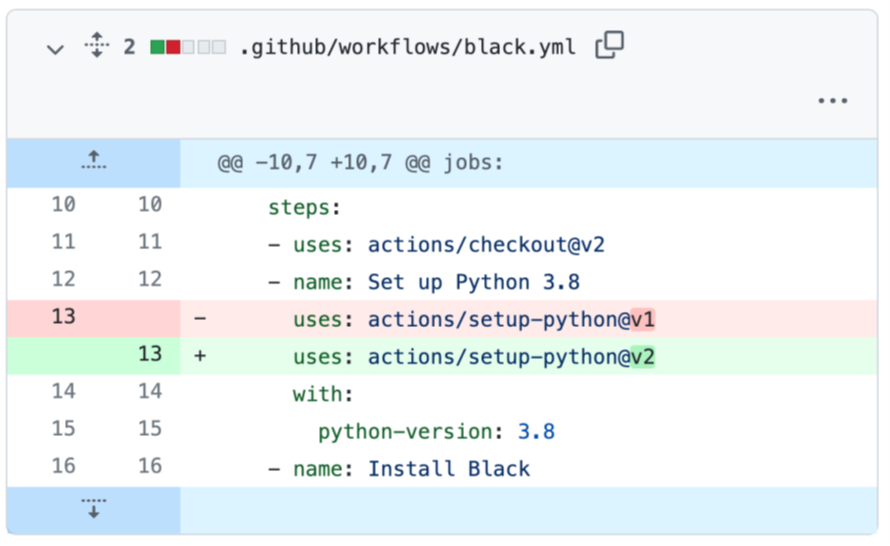
\includegraphics[width=0.5\textwidth]{Figure 1.png}
\caption{Modifying python version \cite{valenzuela2022evolution} }
\end{figure}

    \subsection{Security Vulnerabilities}
        Software that depends on open source and free reusable libraries provided by package managers like npm are more likely to be exposed to security vulnerabilities. To quote Zimmermann et al. \cite{zimmermann2019small}, they mention the following: \\

        \textit{"The open nature of npm has boosted its growth, providing over 800,000 free and reusable software packages. Unfortunately, this open nature also causes security risks, as evidenced by recent incidents of single packages that broke or attacked software running on millions of computers.”} \\

        According to Koishybayev et al. \cite{koishybayev2022characterizing}, one example of a similar attack using the GHA ecosystem is to perform deployments based on the attacker’s code by triggering a misconfigured workflow through a new pull request. Since GHA consists of many open-source reusable Actions, workflow and GHA developers need to be extra careful on choosing what packages they depend on for building jobs. It is a good practice to depend on first-party packages and packages from trustworthy maintainers \cite{zimmermann2019small}. \\

        Saroar et al. \cite{saroar2023developers} mentions that even though the GHA platform provides a marketplace for sharing and reusing open-source Actions, there are still many repositories that prefer to maintain their own GitHub Actions locally within their repositories. The survey analysis conducted by the authors revealed some challenges GitHub users face using the Marketplace where 7 out of 25 participants found it difficult to search for products and hard to check product quality (see Figure 2). Saroar et al. \cite{saroar2023developers} quotes one of the participants from the survey: \\

\textit{"Marketplace does not provide an effective way to filter and sort based on quality, version, contributions, etc."}\\

\begin{figure} [h]
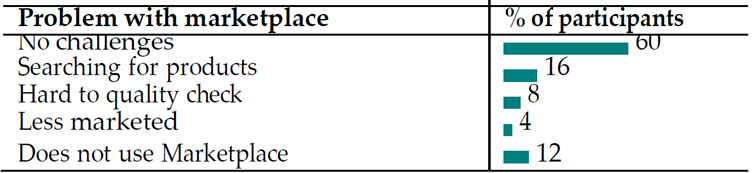
\includegraphics[width=0.5\textwidth]{Table 1.png}
\caption{Challenges found when using GitHub Marketplace \cite{saroar2023developers} }
\end{figure}

	Decan et al. \cite{decan2022use} raised concerns regarding potential issues that might be encountered by GHA, including obsolescence \cite{decan2018evolution} \cite{cogo2021deprecation}, dependency issues \cite{decan2019empirical} \cite{soto2021comprehensive} \cite{decan2019package}, breaking changes \cite{dietrich2019dependency} \cite{decan2018impact}, and security vulnerabilities \cite{zimmermann2019small} \cite{kula2018developers}. These issues have already been faced in reusable software libraries within well-researched ecosystems. In our exploratory study, we aim to investigate whether similar problems also exist within the GHA ecosystem. Moreover, we will compile a list of specific issues from the aforementioned papers and compare our research findings on key issues in GHA with those identified in other ecosystems discussed in the literature. By doing so, we can potentially identify solutions proposed for similar issues in other ecosystems, which could offer insights into addressing the challenges encountered in GHA.\\

	Furthermore, our study aims to build upon the findings of Saroar et al. \cite{saroar2023developers}, providing explanation for their observations regarding the distribution of locally maintained Actions compared to Actions from the marketplace. While the survey conducted by the authors offers valuable insights into the challenges faced when utilizing the GitHub Marketplace, it lacks comprehensive research and comparison involving locally maintained Actions. The primary objective of our research is to evaluate repositories' preferences in utilizing locally maintained Actions versus actions from the GitHub Marketplace. By doing so, we aim to identify and explain the factors that contribute to these preferences and the resulting differences in adoption.



                                                                        %%% RESEARCH MOTHODOLOGY %%%

\section{Research Methodology}
    With this study we aim to answer some of the challenges developers face when building GHA. Our goal is to evaluate whether similar challenges and issues from well-researched reusable libraries can be spotted in the GHA ecosystem.\\

    In this section, we describe the research questions we are trying to answer and the research strategies which will be implemented to facilitate our explorative study. Additionally, we would like to emphasize that we are employing a mixed method study, utilising different data collection and analysis methods that will be described and motivated after each research question. Finally, we identify and explain the limitations relevant to our research.

    \subsection{Research questions and methodology}


        \textbf{RQ1: What factors developers to rely on locally maintained Actions within their repositories, as opposed to utilising Actions available on the GitHub marketplace?}\\

        \textbf{Research Method:}  Repository Mining\\
            
        This research question is answered by measuring similar characteristics of GitHub repositories that utilise GHA. And how these characteristics can correlate with the usage of Local Actions. By quantitatively measuring the size, number of contributors, number of programming languages used, etc. We can make an argument for whether or not the preference for using Local Actions can be tied to project size, complexity, team size, etc.
        \\

        \subsubsection{\textbf{Data Collection}}
	  The study utilizes python scripts\footnote{https://github.com/WalrusArtist/SEM-Thesis/tree/kardo/python} to collect and store repositories using GitHub Actions. Workflow files are fetched from all the stored GitHub repositories using the GitHub API.  The workflow files are then parsed, with each line iterated, to search for the $uses:$ keyword and check whether the reference of the Action matches that of a Marketplace Action or a Local Action. To distinguish between the patterns, we check whether the Action reference matches the pattern $./.github*$. If it does, we determine that it is a Local Action. Similarly, for Marketplace Actions we check whether the Action reference contains the symbol $@$. If it does, we can determine that it is a Marketplace Action. \\ However, an important note here is that developers may have references of Actions that are locally maintained, but kept in other repositories. In this case, an $@$ symbol is present. To fully determine if an Action is indeed from the Marketplace and not from another repository, we applied a step to parse out the Action name, and verify that the Action with the given name exists on the GitHub Marketplace through the GitHub API. \\ Depending on the results, we count the total number of locally maintained actions and GHAs from the marketplace across 4483 repositories to reach a conclusion.\\

	The survey targets audiences who are active GitHub users engaged in software development and GHA. The survey will be distributed through platforms such as Reddit, Stack Overflow, Discord channels, and GitHub repositories, etc. The designed questionnaire collects demographic information, usage patterns of GHA, and factors influencing the selection of actions. Our goal was to collect responses from at least 25-30 participants. The questionnaire was designed according to the following criteria:\\
 \begin{itemize}
	\item Questions are clear and unambiguous.
	\item Questions are relevant to our research question.
	\item Questions are designed to be neutral and free of biases.
	\item Questions are specific and focused on a single topic.
	\item The survey was pilot-tested before administration.\\
 \end{itemize}
Appendix A contains the questions from our survey.\\
        \subsubsection{\textbf{Data Analysis}}
            In the analysis phase, the intent is to utilize both descriptive and inferential statistical techniques to rigorously scrutinize the survey data.  This entails establishing specific criteria for analysis, including the definition of metrics such as the frequency of marketplace action usage, rationales underlying action selection, and the perceived advantages and disadvantages associated with these selections. Moreover, the evaluation process will involve a meticulous examination of emerging trends and the identification of factors shaping distribution patterns.\\

        \textbf{RQ2: In what ways do the key issues encountered in GHA parallel those found in other software ecosystems?}\\

        \textbf{Research Method:} Repository Mining\\

        We are already aware of the problems encountered in other ecosystems. Our goal is to identify similar challenges and/or issues within the GHA ecosystem and evaluate the impact of these problems.\\

       To address RQ2, we plan to carry out repository mining. Through repository mining, we can collect vast amounts of data from relevant software repositories using GHA. We can also automate the process of mining data by developing scripts\footnote{https://github.com/WalrusArtist/SEM-Thesis/tree/kardo/python}  and easing the process of going through multiple repositories \cite{chaturvedi2013tools}.\\

        \subsubsection{\textbf{Data Collection}}
            Repository mining is conducted by utilizing APIs and database queries to collect relevant data from Stack Overflow, GitHub Discussions, and other pertinent repositories. To collect data from GitHub discussions, we utilize GraphQL API  in our scripts\footnote{https://github.com/WalrusArtist/SEM-Thesis/tree/kardo/python} to extract and store relevant discussion posts in JSON format. Particularly, we search for all the discussion posts that contain the query string $GitHub Actions$ . Then, the scripts target the following keywords and their synonyms to gather posts that may contain the following relevant problems: \\
\begin{itemize}
	\item \textbf{Obsolescence:} Outdated, Legacy, Deprecat, Phasing out, Obsolete, Unmaintained
	\item \textbf{Dependency issues:} Dependency, conflict, mismatch, Package, Version, Dependency problem, Incompatible dependenc
	\item	\textbf{Breaking changes:} version, incompatible, API changes, Breaking updates, Breaking modifications, Breaking alterations, Disruptive changes
          \item \textbf{Security vulnerabilities:} security, Security flaws, Security risk, Vulnerabilities, Exploit, loopholes, Attack\\
\end{itemize}
	A similar approach is used to collect questions from Stackoverflow using the Stackoverflow API. Our scripts searches for all the questions that are tagged $GitHub-Actions$ and then targets the aforementioned issues and their synonyms. The discussion posts and questions will be analyzed manually, and conclusions about the problems will be drawn.\\

        \subsubsection{\textbf{Data Analysis}}

            In our data analysis approach, we employed repository mining techniques to analyze patterns and trends in StackOverflow posts, GitHub Discussions threads, and repository data obtained through APIs and database queries. Quantitative analysis encompassed descriptive statistics such as visualization methods including heatmaps. For qualitative analysis, our first step was to compile issues from other existing literature and group them into four themes: i) Obsolescence, ii) Dependency issues, iii) Breaking changes, and iv) Security vulnerabilities. Our collected dataset through MSR was already grouped into these themes during data collection where the data was filtered based on the synonyms appearning in the discussion or stackoverflow threads. However, there were cases when we had to map the same issue to more than one theme. The reason behind this overlapping is because of the close relation and dependency between these themes. For instance, there might be an issue related to security that is a consequence of depending on outdated software packages; in this case the same issue can be grouped to each of these themes 'Obsolescence', 'Dependency Issues', and 'Security vulnerabilities'. \\
In our second step of our qualitative analysis, we utilized open coding to divide our collected issues in each theme to identify further relevant sub-themes which captures more than one synonym and labelled the issues using a list of synonym terms that appears on the sub-themes. We found that the posts that contain more than one term from the synonyms were more relevant to the theme. Then, we utilized axial coding to find patterns and relation between the themes. For instance, if a specific issue from a particular theme is also relevant to other themes,  we added the related theme to the list of synonyms labelling the relation between one or two themes. Our thematic coding is visually presented in Table 1.\\
In summary, our qualitative analysis contained four main themes labelled with the keywords  'Obsolescence', 'Dependency Issues', and 'Security vulnerabilities' and smaller sub-themes labelled with a list of synonyms and related themes. An example of such a list would be $['Outdated', 'Legacy', 'Dependency Issues' ]$. Overall, our approach aimed to provide a comprehensive understanding of the challenges in the GHA ecosystem parallel to other software ecosystems.\\
\begin{tabular}{|c|c|}
  \hline
  \textbf{Main themes} & \textbf{Sub-themes} \\
  \hline
  \hline
    Security Vulnerabilities & Cell 2  \\
  \hline
   Dependency changes & Cell 6 \\
  \hline
  \hline
   Obsolescence & Cell 6 \\
  \hline
  \hline
   Breaking Changes & Cell 6 \\
  \hline
\end{tabular}

        These methods ensure a systematic approach to address each research question effectively.\\

    \subsection{Time Plan}
        The table bellow gives a high level overview of the time plan. A SCRUM framework will be in use throughout the management of the research. 
        \begin{table}[h]
            \centering
            \caption{Project Sprint Timeline}
            \label{tab:sprint_timeline}
            \begin{tabular}{|c|p{0.7\linewidth}|}
            \hline
            \textbf{Sprints} & \textbf{Activities} \\ \hline
            1 and 2  & Design base structure for data collection:
            \begin{itemize}
	      \item (25/03/2024 - 05/04/2024)
                \item Surveys
                \item API scripts
                \item Database Queries
                \item Document and write the literature
            \end{itemize} \\ \hline
            3 and 4  & Collect data based using the instruments designed in sprints 1 and 2:
            \begin{itemize}
                \item  (08/04/2024 - 19/04/2024) 
                \item Send out surveys
                \item Run and gather data from API calls and queries
                \item Document and write the literature
            \end{itemize} \\ \hline
            5 and 6   & Analyse the data collected from sprints 3 and 4:
            \begin{itemize}
                \item(22/04/2024 - 03/05/2024)
                \item Wrap up data collection
                \item Detect patterns
                \item Identify key factors
                \item Draw conclusions
                \item Document and write the literature
            \end{itemize} \\ \hline
            7 and 8   & Refine and finalize the analysis and ensure the literature is clear and concise. 
	  \begin{itemize}
                \item(06/05/2024 - 22/05/2024)
            \end{itemize} \\ \hline
            \end{tabular}
        \end{table}

    \subsection{Threats to Validity}
        In this section, we discuss the limitations and threats to
        validity and how we can mitigate them.\\

        \textbf{External Validity:} Since our repository mining procedure is supposed to collect data from diverse GitHub repositories with different implementation of workflows, programming languages and size of the project, the results we obtain might differ depending on these factors and our findings can’t be generalized for all types of GitHub projects. However, it is possible to group the projects based on their size, programming language, etc. After grouping the projects, we could try to analyse data from each group and identify a common trend between the results to generalize our findings.\\

	\textbf{Construct Validity:} The questionnaire, we are planning to use as our survey instrumentation, might have errors or inconsistencies. The formulated questions might be unclear, ambiguous and/or irrelevant. We could address this risk by adhering to a well-defined criterion for formulating questionnaires. Additionally, we could conduct pilot testing to validate our survey instrument.\\

        \textbf{Response bias:} Collecting data through online surveys carries some risks and may result in anomalies in our results. Specifically, distributing surveys via social media can lead to invalid responses, and we may also face challenges in obtaining a sufficient number of responses to draw meaningful conclusions. To mitigate these potential limitations, we can consider distributing surveys through highly maintained development platforms or reaching out to potential companies in person. 

							    	      %%%RESULTS%%%

\section{Results}
    This section presents the results of our data collection and analysis.
    The survey has received 8 responses until now and based on the answers we can see that developers prefer to use locally maintained Actions. Our scripts shows the total number of each type of Actions used in all the collected repositories and posts related to each type of Action are collected. These data will be analysed starting from Sprint 5.
    For RQ2, we have successfully collected all the posts and questions, from GitHub Discussions and Stackoverflow respectively, that mentions our target keywords. These data data will be analysed starting from Sprint 5.
    \\

    For RQ1, after collecting data across 4483 GitHub repositories that were on the top one-thousand list of popular repositories for the years throughout 2020, 2021, 2022, 2023 and 2024, we applied a filter to dismiss repositories that did not use any Actions. The number of repositries reduced to 1587. \\ 
    In these repositories, Marketplace Actions consisted of 49.30\% of the total Actions, while the remaining 50.70\% consisted of Local Actions. Although, when analysing the number of times each Action was referenced in other parts of the workflow, we found that 60.39\% of the references were from Local Actions and the remaining 39.61\% were from Marketplace Actions. This indicates that Local Actions were more resued than Marketplace Actions. 
    \\

    Data on number of different programming languages, repository size, number of contributors, date of repository creation and bytes of source code were also collected in order to see if there were any correlations between these repository attributes and the amount of Marketplace or Local Actions used or referenced.\\
    Using the Pearson correlation coefficient (PCC) method for this purpose, we found that no strong correlations were found, but there were two moderate correlations between the the number of programming languages and the number of Local Actions were available and referenced. \\
    It's important to mention that when measuring the PCC, we removed outliers from the lower and upper 20\% of repositories that contained very low or very high numbers of Local Actions available and referenced. The effort for removing the outliers was to avoid skewed results. \\

    Number of programming languages used in a repository and the number of Local Actions had a PCC of 0.42. Similarly, the number of programming languages used and the number of times Local Actions were referenced within different parts of the workflow had a PCC of 0.41.


For RQ2, we have found three of four themes that have issues from GHA that can be mapped to issues from other ecosystems. The theme that showed the highest number of mapped issue in GHA was 'Security Vulnerability'. Following this theme were the themes 'Dependency changes' and 'Obsolescence'  that had almost the same number of mapped issue. However, our reasearch work didn't find similar issues in GHA that can be mapped for the theme 'Breaking changes'. Figure 3 and 4 shows a heatmap of the issues found in each of the themes in GitHub Discussions and Stackoverflow before mapping the data. Figure 5 and 6 shows a heatmap of the issues found in each of the themes  in GitHub Discussions and Stackoverflow after mapping the data.



\subsection{Security Vulnerability}
\begin{tabular}{|c|c|}
  \hline
  \textbf{Other Ecosystems} & \textbf{GHA} \\
  \hline
  \hline
    Cell 1 & Cell 2  \\
  \hline
    Cell 3 & Cell 6 \\
  \hline
 
\end{tabular}
\subsection{Obsolescence}
\begin{tabular}{|c|c|}
  \hline
  \textbf{Other Ecosystems} & \textbf{GHA} \\
  \hline
  \hline
    Cell 1 & Cell 2  \\
  \hline
    Cell 2 & Cell 6 \\
  \hline

\end{tabular}
\subsection{Dependency changes}
\begin{tabular}{|c|c|}
  \hline
  \textbf{Other Ecosystems} & \textbf{GHA} \\
  \hline
  \hline
    Cell 1 & Cell 2  \\
  \hline
   Cell 3 & Cell 6 \\
  \hline

\end{tabular}
\subsection{Breaking changes}
\begin{tabular}{|c|c|}
  \hline
  \textbf{Other Ecosystems} & \textbf{GHA} \\
  \hline
  \hline
    Cell 1 & Cell 2  \\
  \hline
   Cell 3& Cell 6 \\
  \hline
\end{tabular}
							    	      %%%DISCUSSION%%%

\section{Conclusion}
	
In this section, we discuss the results in conjunction with relevant literature.

\section{Future work}
							    %%% ACKNOWLEDGEMENT %%%

\section{Acknowledgement}

         This proposal is the collaborative effort of Kardo Marof and Saif Sayed, with guidance from our thesis supervisor, Linda Erlenhov. Marof's contributions include the Introduction section, as well as the sub-sections on Data Collection and Data Analysis within the Research Methodology section. Sayed, on the other hand, contributed to the Related Works section, the description of the Research Questions, the motivation behind the selected methodologies, and the identification of Threats to Validity within the Research Methodology section.

							           %%% APPENDICES%%%

\section{Appendices}

                                                                             %%% REFERENCES %%%
\bibliographystyle{unsrt}
\bibliography{references}

\vspace{12pt}
\end{document}
